\chapter{Data}

Our main source of data is the Cantus database (\cite{cantus_db}), one of the databases indexed in the Cantus Index. The database serves as a 
digital archive of chants, each entry containing information about its source, liturgical occasion, mode, and others. Work on the project started
in the late 1980s, and to date, around 500,000 individual chants from approximately 150 manuscripts have been indexed. Each entry is transcribed 
manually and undergoes a thorough examination before publishing (\cite{cantus_lacoste}).

We are using a scraped version of the Cantus database released as CantusCorpus (\cite(chant21)). Unlike the Cantus database which is continuously being
updated and is therefore unsuitable for computational study, the corpus is versioned, therefore each version always contains the same data. We are using
version 0.2 released in July 2020 which contains 497,071 entries. However, a majority of the data is not suitable for this application, as they do not
contain all the necessary fields, therefore we are only using a subset of size around 13,000. The corpus is available for download in CSV format.

\section{CSV}

CSV is one of the most common formats for tabular data. The abbreviation stands for \emph{comma-separated values}. As the name suggests, the format
uses commas to separate columns (although other separators, such as a semicolon, can be used as well to allow for simpler parsing in case that the data 
frequently contains commas that would otherwise need to be escaped), while the individual rows are separated by a line break. The data is stored as plaintext,
which makes it easily readable. Parsing CSV files becomes more complicated when the data contains column and row separators inside fields; in that case
quotation marks or esape sign has to be used. There exist many well-designed parsers, one such parser is the Python module simply called \emph{csv}.
This application uses the module \emph{pandas} to parse CSV files, which in turn uses the \emph{csv} module.

\section{Database fields}

The following table represents the data fields in the database.

\begin{longtable}{| p{.25\textwidth} | p{.75\textwidth} |} 
%\begin{center}
%\begin{tabular}{| c | c |} 

 \hline
 Data field & Description \\
 \hline
 id             & automatically generated id in the database \\ \hline
 corpus\_id     & human-readable id identifying the chant in the CantusCorpus \\ \hline
 incipit        & incipit (the first few words) of chant \\ \hline
 cantus\_id     & id identifying the chant in the Cantus Index \\ \hline
 mode           & mode of the chant \\ \hline
 finalis        & the final note of the chant \\ \hline
 differentia    & the melodic ending of psalms \\ \hline
 siglum         & manuscript in which the chant is found \\ \hline
 position       & liturgical role of the chant \\ \hline
 folio          & page of the manuscript where the chant is found \\ \hline
 sequence       & order in which the chant is found in the folio \\ \hline
 marginalia     & clarification about the location of the chant \\ \hline
 cao\_concordances & FILL IN \\ \hline
 feast\_id      & feast of the year during which the chant was sung \\ \hline
 genre\_id      & genre of the chant, e.g. \emph{antiphon}, \emph{responsory} \\ \hline
 office\_id     & office of the day during which the chant was sung, e.g. \emph{Laudes}, \emph{Vespers} \\ \hline
 source\_id     & id of the manuscript in which the chant is found \\ \hline
 melody\_id     & id of melody by which it can be found in the Cantus Index \\ \hline
 drupal\_path   & URL of the chant on the Cantus database website \\ \hline
 full\_text     & full text in a standardized spelling \\ \hline
 full\_text\_manuscript & full text in the manuscript spelling \\ \hline
 volpiano       & transcription of the melody in volpiano format \\ \hline
 notes          & indexing notes \\
 \hline

%\end{tabular}
%\end{center}
\caption{List of database fields}
\end{longtable}

\section{User-defined data}

The application enables user to upload their own dataset. The following table specifies the fields in the database. If a CSV in an
incorrect format is uploaded (e.g. the required fields are empty), the application will not work properly. The meaning of the individual
fields is as described in the previous section unless said otherwise.

\begin{longtable}{| p{.3\textwidth} | p{.15\textwidth} | p{.1\textwidth} | p{.45\textwidth} |} 
%\begin{center}
%\begin{tabular}{| c | c | c | c |} 

 \hline
 Column name     & Type  & Can be empty  & Notes \\
 \hline
 \emph{none} \emph{or} Unnamed: 1 & any & yes & the column will be dropped  \\ \hline
 id             & string & yes & equivalent to \emph{corpus\_id} in the database \\ \hline
 incipit        & string & no  & \\ \hline
 cantus\_id     & string & yes & should be a valid Cantus ID \\ \hline
 mode           & string & yes & list of modes is in attachment \\ \hline
 finalis        & string & yes & \\ \hline
 differentia    & string & yes & \\ \hline
 siglum         & string & yes & \\ \hline
 position       & string & yes & \\ \hline
 folio          & string & yes & \\ \hline
 sequence       & string & yes & \\ \hline
 marginalia     & string & yes & \\ \hline
 cao\_concordances & string & yes & \\ \hline
 feast\_id      & string & yes & list of feasts is in attachment \\ \hline
 genre\_id      & string & yes & list of genres is in attachment \\ \hline
 office\_id     & string & yes & list of offices is in attachment \\ \hline
 source\_id     & string & yes & \\ \hline
 melody\_id     & string & yes & \\ \hline
 drupal\_path   & string & yes & should be a valid URL \\ \hline
 full\_text     & string & no  & \\ \hline
 full\_text\_manuscript & string & yes & \\ \hline
 volpiano       & string & no  & has to be in Volpiano format \\ \hline
 notes          & string & yes & \\
 \hline

%\end{tabular}
%\end{center}
\caption{Fields in the user-uploaded CSV}
\end{longtable}

\begin{figure}[h]
    \begin{lstlisting}[breaklines]
    ,id,incipit,cantus_id,mode,finalis,differentia,siglum,position,folio,sequence,marginalia,cao_concordances,feast_id,genre_id,office_id,source_id,melody_id,drupal_path,full_text,full_text_manuscript,volpiano,notes
    621,chant_000622,A Christo de caelo vocatus,001188,8,,1,F-Pn lat. 12044,3.,053v,5.0,,,feast_0287,genre_a,office_m,source_014,,http://cantus.uwaterloo.ca/chant/399542/,A Christo de caelo vocatus et in terram prostratus ex persecutore effectus est vas electionis,A xpisto de caelo vocatus et in terram prostratus ex persequutore effectus est vas electionis,1---g---g-kk--h---g---h--g---f--gh--g---g---g---hgf--g---gh--f--f7---g---f--h--j--kl--kj-klk---h--kj--hg---g---h---gf--gh--h--g--g---4,
    635,chant_000636,A Christo de caelo vocatus,007123a,1,,,US-CHNbcbl 097,01,035r,2.0,,,feast_1321,genre_v,office_m,source_069,,http://cantus.uwaterloo.ca/chant/665425/,A Christo de caelo vocatus,,1--h---h--hghgf---g---g--g---g--gh--g---,
    645,chant_000646,A Christo de caelo vocatus,007123a,1,,,D-KA Aug. LX,01,125r,2.0,,,feast_1321,genre_v,office_m,source_414,,http://cantus.uwaterloo.ca/chant/617583/,A Christo de caelo vocatus et in terram prostratus ex persecutore effectus est vas electionis,A xpisto de celo vocatus et in terram prostratus ex persecutore effectus est vas electionis | ~Vere,1---h-h---hg--hg-gf7---g---g--g---g--gh--g---g---g---hG--gh---gh--hjh--h---hf---gh--h--h--hk--h---h--hk--h---h---h---hg-hg--hf--fghg--hkh-hgfe--fgh-gf7---3,
    667,chant_000668,A Christo de caelo vocatus,007123a,1,,,A-KN 1018,01,071v,3.0,,,feast_1321,genre_v,office_m,source_265,,http://cantus.uwaterloo.ca/chant/293103/,A Christo de caelo vocatus et in terram prostratus ex persecutore effectus est vas electionis,A christo de celo vocatus et in terram prostratus ex persecutore efectus est vas eleccionis,1---dh---h--hg-hgg---g---g--g---g--gh--g---g---g---hF--gh7---gh--hijh--h---h---gH--h--h--hk--h---h--hk--h---h---hghgfed-efg---gh--fe7--ef--fghgh--gf---3,
    923,chant_000924,A deo praelectus*,600006,8,,,NL-Uu 406,,196r,8.0,,,feast_1814,genre_r,office_v2,source_573,,http://cantus.uwaterloo.ca/chant/497010/,A deo praelectus*,A deo preelectus,1---g---g--ffg---gge---3,
    \end{lstlisting}
\caption{Example of a valid CSV file}
\end{figure}

\section{Volpiano}

The melodies in the volpiano fields are encoded as strings of alphanumeric characters and dashes. These can be rendered as musical notation using
the volpiano font. Each character represents either a pitch, empty space, or other musical characters, such as a clef.

Volpiano was developed as a research tool optimized for databases and word processors. There are strict rules concerning the transcription, which leads
to all volpiano-encoded melodies having a standardized format. Each transcription begins with a treble clef. Gaps between words are encoded as three
dashes, while two dashes represent gaps between syllables (\cite{volpiano}).

\begin{figure}[h]
\centering
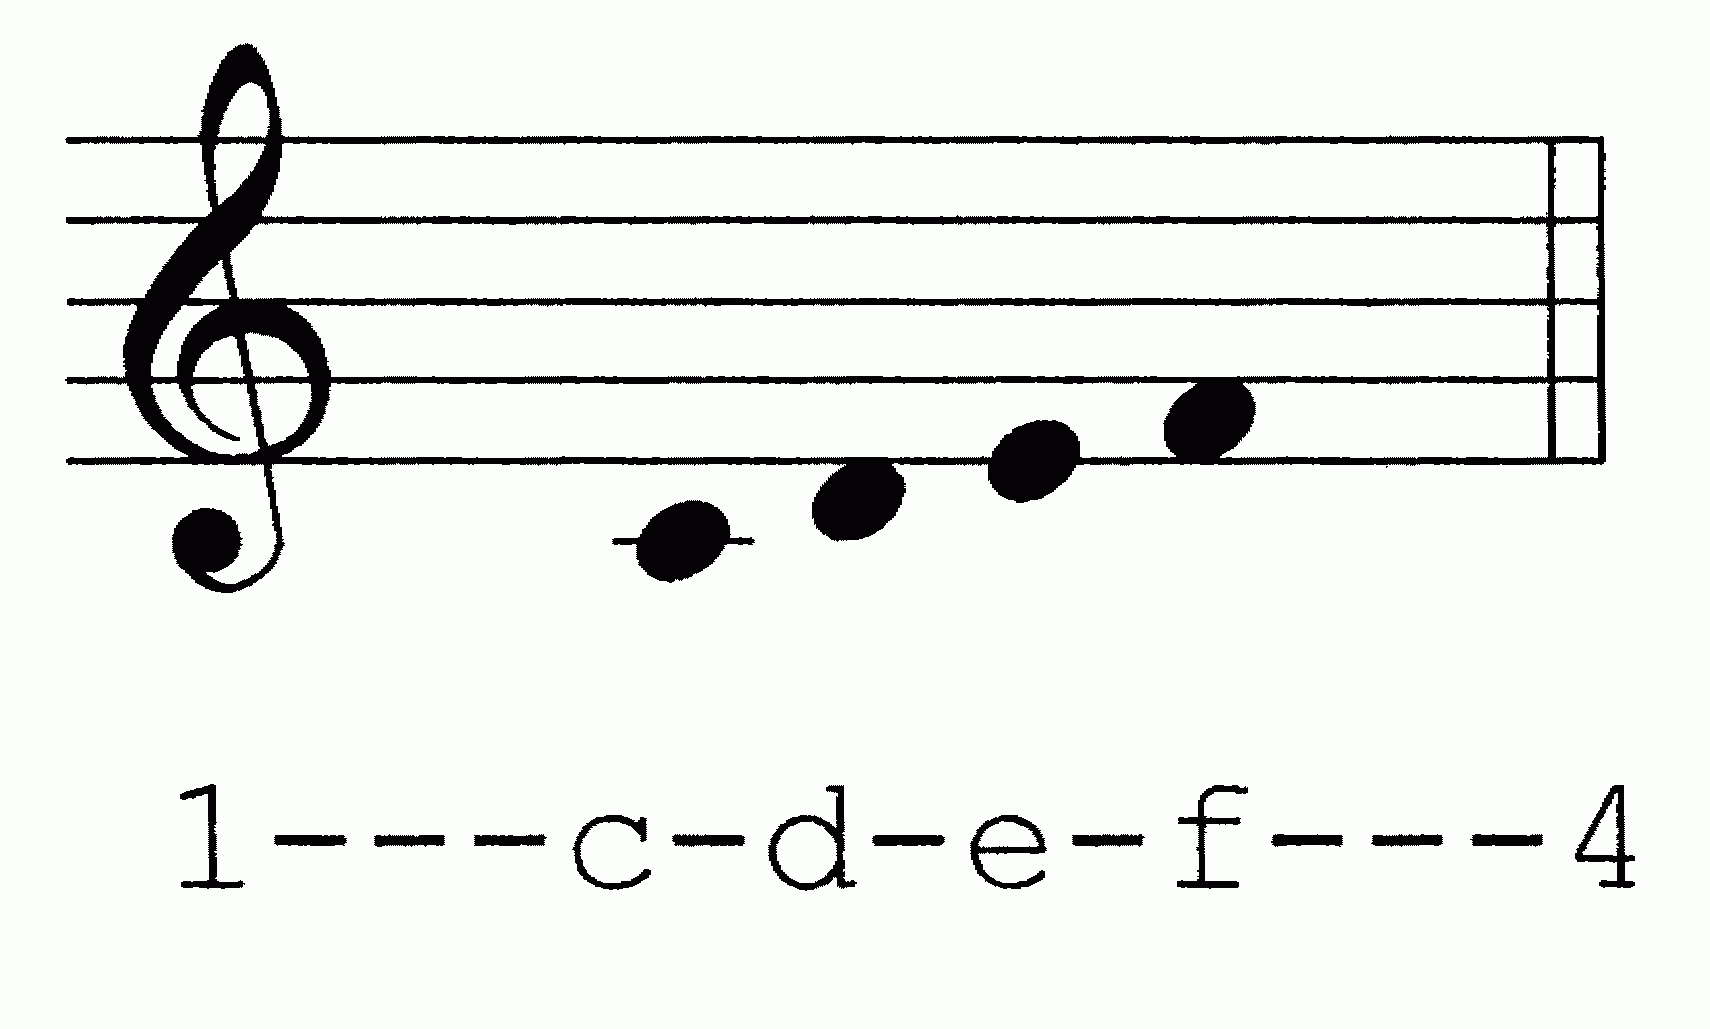
\includegraphics[scale=0.1]{volpiano}
\caption{Example of volpiano as stored in the database and how it is rendered as musical notation. \cite[Figure~2]{cantus_lacoste}}
\end{figure}

\section{Data cleaning}

As mentioned earlier, not the entire dataset is usable. Since we are analysing melodies, it is necessary that each data point contains information
about the chant's melody.

As one of the application's main features is melody alignment, it is necessary that we only use those data points whose \emph{volpiano} field is
not empty. Moreover, some visualizations compare text length to melody length, therefore we require the data points to have both. Additionally, 
text and melody should be able to be aligned, i.e. they contain the same number of words and syllables.

Removing the data that does not adhere to the conditions, we are left with 13,397 usable data points.

